\documentclass[10pt]{beamer}
\usetheme{Madrid}

\setbeamertemplate{bibliography item}[text] % this will create numbering for the references, like [1], [2], ... Without this, the references will still show and will have icons instead of numbers.

\usecolortheme{whale}
\usepackage{graphicx}
\usepackage{amsmath, amssymb, amsthm}
\usepackage{booktabs}
\usepackage{caption}
\usepackage{subcaption}
\usepackage{tikz}
\usetikzlibrary{positioning, shapes, arrows, calc, fit}
\usepackage{algorithm}
\usepackage{algpseudocode}
\usepackage{multirow}
\usepackage{hyperref}

\title{Generative Adversarial Networks}
\subtitle{A Comprehensive Lecture}
\author{Amir}
\institute{Computer Vision}
\date{}

\begin{document}

\begin{frame}
\titlepage
\end{frame}

\begin{frame}{Outline}
\tableofcontents
\end{frame}

\section{Introduction}
\begin{frame}{What are Generative Models?}
\begin{block}{Definition}
Models that learn the underlying probability distribution $p_{data}(x)$ from samples and can generate new samples from this distribution.
\end{block}

\begin{columns}
\begin{column}{0.5\textwidth}
\textbf{Discriminative Models:}
\begin{itemize}
    \item Learn $p(y|x)$
    \item Classify/regress
    \item Decision boundaries
\end{itemize}
\end{column}
\begin{column}{0.5\textwidth}
\textbf{Generative Models:}
\begin{itemize}
    \item Learn $p(x)$ or $p(x|y)$
    \item Generate new data
    \item Understand data structure
\end{itemize}
\end{column}
\end{columns}

\begin{exampleblock}{Applications}
\begin{itemize}
    \item Image synthesis (art, design)
    \item Data augmentation
    \item Anomaly detection
    \item Style transfer
\end{itemize}
\end{exampleblock}
\end{frame}

\begin{frame}{Types of Generative Models}
\begin{figure}
\centering
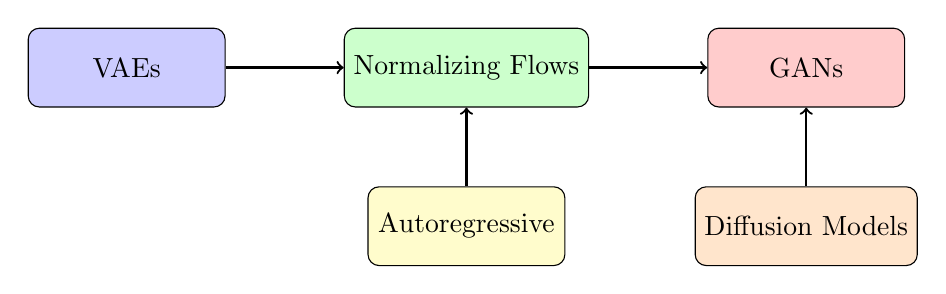
\begin{tikzpicture}[
    node distance=1.5cm,
    box/.style={draw, rectangle, rounded corners, minimum width=2.5cm, minimum height=1cm, text centered}
]
\node[box, fill=blue!20] (vae) {VAEs};
\node[box, fill=green!20, right=of vae] (flow) {Normalizing Flows};
\node[box, fill=red!20, right=of flow] (gan) {GANs};
\node[box, fill=yellow!20, below=1cm of flow] (ar) {Autoregressive};
\node[box, fill=orange!20, below=1cm of gan] (diff) {Diffusion Models};

\draw[->, thick] (vae.east) -- (flow.west);
\draw[->, thick] (flow.east) -- (gan.west);
\draw[->, thick] (ar.north) -- (flow.south);
\draw[->, thick] (diff.north) -- (gan.south);
\end{tikzpicture}
\caption{Evolution of generative models}
\end{figure}

\begin{alertblock}{GAN Characteristics}
\begin{itemize}
    \item \textbf{Adversarial training}: Two networks compete
    \item \textbf{No explicit likelihood}: Implicit distribution learning
    \item \textbf{State-of-the-art}: Best image quality (until diffusion models)
\end{itemize}
\end{alertblock}
\end{frame}

%\section{Fundamentals of GANs}
%\begin{frame}{The GAN Framework}
%\begin{figure}
%\centering
%\begin{tikzpicture}[
%    neuron/.style={circle, draw, minimum size=0.8cm},
%    arrow/.style={->, thick, >=stealth}
%]
%
%% Generator
%\node[neuron, fill=green!20] (noise) {z};
%\node[neuron, fill=green!20, right=1.5cm of noise] (g1) {};
%\node[neuron, fill=green!20, right=1cm of g1] (g2) {};
%\node[neuron, fill=green!30, right=1cm of g2] (gout) {G(z)};
%\node[above=0.2cm of noise] {Noise};
%\node[above=0.2cm of gout] {Fake Data};
%
%% Discriminator
%\node[neuron, fill=blue!20, below right=1.5cm and 0.5cm of gout] (data) {x};
%\node[neuron, fill=blue!20, right=1.5cm of data] (d1) {};
%\node[neuron, fill=blue!20, right=1cm of d1] (d2) {};
%\node[neuron, fill=blue!30, right=1cm of d2] (dout) {D(·)};
%\node[above=0.2cm of data] {Real Data};
%\node[above=0.2cm of dout] {Real/Fake?};
%
%% Arrows
%\draw[arrow] (noise) -- (g1);
%\draw[arrow] (g1) -- (g2);
%\draw[arrow] (g2) -- (gout);
%\draw[arrow] (data) -- (d1);
%\draw[arrow] (d1) -- (d2);
%\draw[arrow] (d2) -- (dout);
%\draw[arrow, dashed] (gout) -- ++(0,-1) -| (d1);
%
%% Labels
%\node[above=0.5cm of g1, font=\small] {Generator (G)};
%\node[above=0.5cm of d1, font=\small] {Discriminator (D)};
%
%\end{tikzpicture}
%\caption{Adversarial training: G tries to fool D, D tries to detect fakes}
%\end{figure}
%\end{frame}

\section{Fundamentals of GANs}
\begin{frame}{The GAN Framework}
\begin{figure}
\centering
% resizebox ensures the diagram stays within the slide margins
\resizebox{0.9\textwidth}{!}{
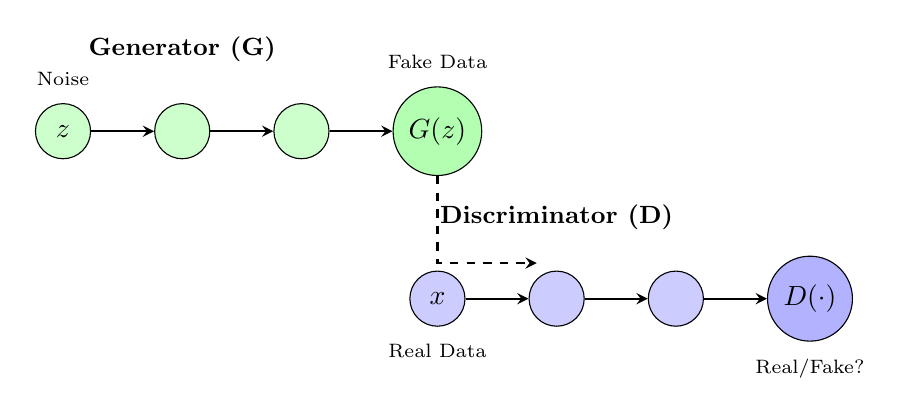
\begin{tikzpicture}[
    neuron/.style={circle, draw, minimum size=0.7cm},
    arrow/.style={->, thick, >=stealth},
    node distance=0.8cm and 0.8cm
]

% --- Generator (G) ---
\node[neuron, fill=green!20] (noise) {$z$};
\node[neuron, fill=green!20, right=of noise] (g1) {};
\node[neuron, fill=green!20, right=of g1] (g2) {};
\node[neuron, fill=green!30, right=of g2] (gout) {$G(z)$};

\node[above=0.1cm of noise, font=\scriptsize] {Noise};
\node[above=0.1cm of gout, font=\scriptsize] {Fake Data};
\node[above=0.4cm of g1, font=\small\bfseries] {Generator (G)};

% --- Discriminator (D) ---
% Positioned below and slightly shifted to save horizontal space
\node[neuron, fill=blue!20, below=1.2cm of gout] (data) {$x$};
\node[neuron, fill=blue!20, right=of data] (d1) {};
\node[neuron, fill=blue!20, right=of d1] (d2) {};
\node[neuron, fill=blue!30, right=of d2] (dout) {$D(\cdot)$};

\node[below=0.1cm of data, font=\scriptsize] {Real Data};
\node[below=0.1cm of dout, font=\scriptsize] {Real/Fake?};
\node[above=0.4cm of d1, font=\small\bfseries] {Discriminator (D)};

% --- Arrows ---
\draw[arrow] (noise) -- (g1);
\draw[arrow] (g1) -- (g2);
\draw[arrow] (g2) -- (gout);

\draw[arrow] (data) -- (d1);
\draw[arrow] (d1) -- (d2);
\draw[arrow] (d2) -- (dout);

% Connecting G output to D input
\draw[arrow, dashed] (gout) |- ([yshift=0.2cm]d1.north west);

\end{tikzpicture}
}
\caption{Adversarial training: G tries to fool D, D tries to detect fakes}
\end{figure}
\end{frame}


\section{Fundamentals of GANs}
\begin{frame}{The GAN MiniMax Game}

\begin{columns}[T]
    % Column 1: Concept Text
    \begin{column}{0.45\textwidth}
    \small
    A GAN is a \textbf{two-player minimax game} played between $G$ and $D$:
    \begin{itemize}
        \item \textbf{Generator ($G$)}: Tries to minimize the probability that $D$ identifies its samples as fake.
        \item \textbf{Discriminator ($D$)}: Tries to maximize the probability of correctly labeling real vs. fake data.
    \end{itemize}
    \end{column}

    % Column 2: Compressed Diagram
    \begin{column}{0.5\textwidth}
    \centering
    \resizebox{\textwidth}{!}{
    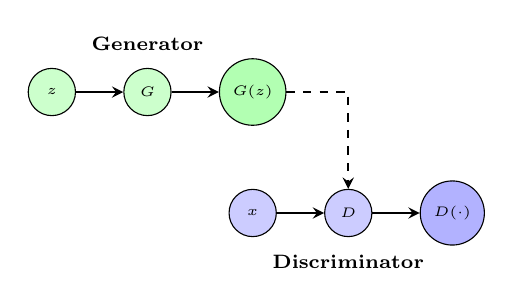
\begin{tikzpicture}[
        neuron/.style={circle, draw, minimum size=0.6cm, font=\tiny},
        arrow/.style={->, thick, >=stealth},
        node distance=0.6cm
    ]
    % G Network
    \node[neuron, fill=green!20] (z) {$z$};
    \node[neuron, fill=green!20, right=of z] (g) {$G$};
    \node[neuron, fill=green!30, right=of g] (gz) {$G(z)$};
    
    % D Network
    \node[neuron, fill=blue!20, below=0.8cm of gz] (x) {$x$};
    \node[neuron, fill=blue!20, right=of x] (d) {$D$};
    \node[neuron, fill=blue!30, right=of d] (dout) {$D(\cdot)$};
    
    % Connections
    \draw[arrow] (z) -- (g); \draw[arrow] (g) -- (gz);
    \draw[arrow] (x) -- (d); \draw[arrow] (d) -- (dout);
    \draw[arrow, dashed] (gz) -| (d);
    
    \node[above=0.1cm of g, font=\scriptsize\bfseries] {Generator};
    \node[below=0.1cm of d, font=\scriptsize\bfseries] {Discriminator};
    \end{tikzpicture}
    }
    \end{column}
\end{columns}

\vspace{0.3cm}

\begin{block}{Original GAN Objective \cite{goodfellow2014gan}}
\[
\min_G \max_D V(D, G) = \mathbb{E}_{x \sim p_{data}(x)}[\log D(x)] + \mathbb{E}_{z \sim p_z(z)}[\log(1 - D(G(z)))]
\]
\end{block}

\centering
\scriptsize \textit{Both models are trained simultaneously in a competition to reach a Nash Equilibrium.}
\end{frame}


\begin{frame}{Nash Equilibrium in GANs}
\begin{itemize}
    \item In the GAN minimax game, the training process seeks a \textbf{Nash Equilibrium} where neither player can improve their outcome by changing their strategy.
    \item This point is reached when the generator produces the true data distribution: $p_g = p_{data}$.
\end{itemize}

\begin{block}{Optimal Discriminator and Equilibrium}
At the equilibrium point, the discriminator is unable to distinguish between real and fake data, resulting in:
\[
D^*(x) = \frac{p_{data}(x)}{p_{data}(x) + p_g(x)} = \frac{1}{2}
\]
\end{block}

\begin{itemize}
    \item \textbf{Global Minimum:} Goodfellow et al. \cite{goodfellow2014gan} proved that the global minimum of the training criterion is achieved if and only if $p_g = p_{data}$.
    \item \textbf{Challenge:} In practice, finding the Nash Equilibrium is difficult because gradient descent is designed to find local minima of a function, not a stationary point in a game.
\end{itemize}

%\vfill
%\tiny
%\bibliographystyle{plain}
%\bibliography{references}
\end{frame}


\begin{frame}{Mathematical Formulation}
\begin{block}{Original GAN Objective \cite{goodfellow2014gan}}
\[
\min_G \max_D V(D, G) = \mathbb{E}_{x \sim p_{data}(x)}[\log D(x)] + \mathbb{E}_{z \sim p_z(z)}[\log(1 - D(G(z)))]
\]
\end{block}

\begin{columns}
\begin{column}{0.5\textwidth}
\textbf{Discriminator:}
\begin{itemize}
    \item Maximizes $V(D,G)$
    \item Distinguishes real from fake
    \item Outputs probability (0 to 1)
\end{itemize}
\end{column}
\begin{column}{0.5\textwidth}
\textbf{Generator:}
\begin{itemize}
    \item Minimizes $V(D,G)$
    \item Maximizes $\log D(G(z))$
    \item Learns to fool D
\end{itemize}
\end{column}
\end{columns}

\begin{theorem}[Optimal Discriminator]
For fixed G, the optimal discriminator is:
\[
D^*(x) = \frac{p_{data}(x)}{p_{data}(x) + p_g(x)}
\]
\end{theorem}
\end{frame}

\begin{frame}{Training Algorithm}
\begin{algorithm}[H]
\caption{GAN Training Algorithm}
\begin{algorithmic}[1]
\Require Learning rates $\alpha_D$, $\alpha_G$, number of iterations $N$
\Require $k$: number of D steps per G step
\For{iteration = 1 to $N$}
    \For{$t = 1$ to $k$}
        \State Sample minibatch $\{x^{(i)}\}_{i=1}^m \sim p_{data}$
        \State Sample minibatch $\{z^{(i)}\}_{i=1}^m \sim p_z$
        \State Update D: $\theta_D \leftarrow \theta_D + \alpha_D \nabla_{\theta_D} \frac{1}{m} \sum_{i=1}^m [\log D(x^{(i)}) + \log(1 - D(G(z^{(i)})))]$
    \EndFor
    \State Sample minibatch $\{z^{(i)}\}_{i=1}^m \sim p_z$
    \State Update G: $\theta_G \leftarrow \theta_G - \alpha_G \nabla_{\theta_G} \frac{1}{m} \sum_{i=1}^m \log(1 - D(G(z^{(i)})))$
\EndFor
\end{algorithmic}
\end{algorithm}

\begin{alertblock}{Practical Note}
In practice, update G to maximize $\log D(G(z))$ instead of minimizing $\log(1 - D(G(z)))$ to avoid vanishing gradients early in training.
\end{alertblock}
\end{frame}

\section{Deep Dive into GAN Mathematics}
\begin{frame}{Optimal Discriminator Derivation}
For fixed G, we want to maximize:
\[
V(D) = \mathbb{E}_{x \sim p_{data}}[\log D(x)] + \mathbb{E}_{z \sim p_z}[\log(1 - D(G(z)))]
\]

Rewrite as integral:
\[
V(D) = \int_x p_{data}(x) \log D(x) + p_g(x) \log(1 - D(x)) dx
\]

Take functional derivative w.r.t $D(x)$ and set to zero:
\[
\frac{\partial V}{\partial D(x)} = \frac{p_{data}(x)}{D(x)} - \frac{p_g(x)}{1 - D(x)} = 0
\]

Solve for $D(x)$:
\[
D^*(x) = \frac{p_{data}(x)}{p_{data}(x) + p_g(x)}
\]
\end{frame}

\begin{frame}{Global Optimality and Convergence}
Substitute $D^*(x)$ into value function:
\begin{align*}
C(G) &= \max_D V(G, D) \\
&= \mathbb{E}_{x \sim p_{data}}[\log D^*(x)] + \mathbb{E}_{x \sim p_g}[\log(1 - D^*(x))] \\
&= \mathbb{E}_{x \sim p_{data}}\left[\log\frac{p_{data}(x)}{p_{data}(x) + p_g(x)}\right] + \mathbb{E}_{x \sim p_g}\left[\log\frac{p_g(x)}{p_{data}(x) + p_g(x)}\right]
\end{align*}

This equals:
\[
C(G) = -\log 4 + 2 \cdot JSD(p_{data} \| p_g)
\]
where JSD is Jensen-Shannon divergence.

\begin{theorem}
The global minimum of $C(G)$ is achieved if and only if $p_g = p_{data}$.
\end{theorem}
\end{frame}

\section{Challenges and Solutions}
\begin{frame}{Training Instability: Common Issues}
\begin{columns}
\begin{column}{0.5\textwidth}
\begin{block}{Vanishing Gradients}
\begin{itemize}
    \item D becomes too good too fast
    \item $\log(1 - D(G(z))) \to 0$
    \item G gets no useful gradient
\end{itemize}
\end{block}

\begin{block}{Mode Collapse}
\begin{itemize}
    \item G produces limited variety
    \item Captures few modes of $p_{data}$
    \item Diversity loss
\end{itemize}
\end{block}
\end{column}

\begin{column}{0.5\textwidth}
\begin{block}{Non-Convergence}
\begin{itemize}
    \item Oscillations in loss
    \item No equilibrium reached
    \item Cyclic behavior
\end{itemize}
\end{block}

\begin{figure}
\centering
\includegraphics[width=\textwidth]{images/mode_collapse.png}
\caption{Mode collapse example}
\end{figure}
\end{column}
\end{columns}
\end{frame}

\begin{frame}{Wasserstein GAN (WGAN) \cite{arjovsky2017wgan}}
\begin{block}{Key Insight}
Use Earth Mover (Wasserstein-1) distance instead of JS divergence:
\[
W(p_{data}, p_g) = \inf_{\gamma \in \Pi(p_{data}, p_g)} \mathbb{E}_{(x,y) \sim \gamma}[\|x - y\|]
\]
\end{block}

\begin{block}{Kantorovich-Rubinstein Duality}
\[
W(p_{data}, p_g) = \sup_{\|f\|_L \leq 1} \mathbb{E}_{x \sim p_{data}}[f(x)] - \mathbb{E}_{x \sim p_g}[f(x)]
\]
\end{block}

\begin{block}{WGAN Objective}
\[
\min_G \max_{D \in \mathcal{D}} \mathbb{E}_{x \sim p_{data}}[D(x)] - \mathbb{E}_{z \sim p_z}[D(G(z))]
\]
where $\mathcal{D}$ is set of 1-Lipschitz functions.
\end{block}
\end{frame}

\begin{frame}{WGAN-GP: Gradient Penalty \cite{gulrajani2017wgangp}}
\begin{block}{Problem with Weight Clipping}
Enforcing Lipschitz via weight clipping leads to:
\begin{itemize}
    \item Capacity underuse
    \item Exploding/vanishing gradients
\end{itemize}
\end{block}

\begin{block}{Gradient Penalty Solution}
Add penalty term:
\[
L = \underbrace{\mathbb{E}_{\tilde{x} \sim p_g}[D(\tilde{x})] - \mathbb{E}_{x \sim p_{data}}[D(x)]}_{\text{Wasserstein loss}} + \lambda \underbrace{\mathbb{E}_{\hat{x} \sim p_{\hat{x}}}[(\|\nabla_{\hat{x}} D(\hat{x})\|_2 - 1)^2]}_{\text{Gradient penalty}}
\]
\end{block}

\begin{alertblock}{Improved Stability}
\begin{itemize}
    \item Better gradient flow
    \item Higher quality samples
    \item More stable training
\end{itemize}
\end{alertblock}
\end{frame}

\section{Important GAN Variants}
\begin{frame}{DCGAN: Deep Convolutional GAN \cite{radford2015dcgan}}
\begin{columns}
\begin{column}{0.5\textwidth}
\begin{block}{Architecture Guidelines}
\begin{enumerate}
    \item Replace pooling with strided convolutions
    \item Use BatchNorm in both G and D
    \item Remove fully connected layers
    \item Use ReLU (G) and LeakyReLU (D)
\end{enumerate}
\end{block}
\end{column}

\begin{column}{0.5\textwidth}
\begin{figure}
\centering
\includegraphics[width=\textwidth]{images/dcgan_architecture.png}
\caption{DCGAN generator architecture}
\end{figure}
\end{column}
\end{columns}

\begin{exampleblock}{Key Contributions}
\begin{itemize}
    \item First stable CNN-based GAN
    \item Learned meaningful latent representations
    \item Vector arithmetic in latent space
\end{itemize}
\end{exampleblock}
\end{frame}

%\begin{frame}{Conditional GANs \cite{mirza2014cgan}}
%\begin{block}{Objective Function}
%\[
%\min_G \max_D V(D, G) = \mathbb{E}_{x \sim p_{data}}[\log D(x|y)] + \mathbb{E}_{z \sim p_z}[\log(1 - D(G(z|y)|y))]
%\]
%\end{block}
%
%\begin{figure}
%\centering
%\begin{tikzpicture}[
%    node distance=0.8cm,
%    box/.style={draw, rectangle, minimum height=0.8cm}
%]
%\node[box] (z) {z};
%\node[box, right=of z] (y) {y};
%\node[box, right=of y] (concat) {[z; y]};
%\node[box, right=of concat] (g) {G};
%\node[box, right=of g] (gout) {G(z|y)};
%\node[box, below=1.5cm of gout] (x) {x};
%\node[box, right=of x] (y2) {y};
%\node[box, right=of y2] (concat2) {[x; y]};
%\node[box, right=of concat2] (d) {D};
%\node[box, right=of d] (dout) {Real/Fake};
%
%\draw[->] (z) -- (concat);
%\draw[->] (y) -- (concat);
%\draw[->] (concat) -- (g);
%\draw[->] (g) -- (gout);
%\draw[->] (gout) -- ++(0,-1.5) -| (concat2);
%\draw[->] (x) -- (concat2);
%\draw[->] (y2) -- (concat2);
%\draw[->] (concat2) -- (d);
%\draw[->] (d) -- (dout);
%\end{tikzpicture}
%\caption{cGAN architecture: conditioning on both generator and discriminator}
%\end{figure}
%\end{frame}

\begin{frame}{Conditional GANs \cite{mirza2014cgan}}

\begin{columns}[T]
    % Column 1: The Equation
    \begin{column}{0.5\textwidth}
    \begin{block}{Objective Function}
    \small
    \[ \min_G \max_D V(D, G) = \]
    \[ \mathbb{E}_{x \sim p_{data}}[\log D(x|y)] + \]
    \[ \mathbb{E}_{z \sim p_z}[\log(1 - D(G(z|y)|y))] \]
    \end{block}
    \footnotesize
    Unlike standard GANs, both $G$ and $D$ receive auxiliary information $y$ (e.g., class labels or images).
    \end{column}

    % Column 2: The Diagram
    \begin{column}{0.45\textwidth}
    \centering
    \resizebox{\textwidth}{!}{
    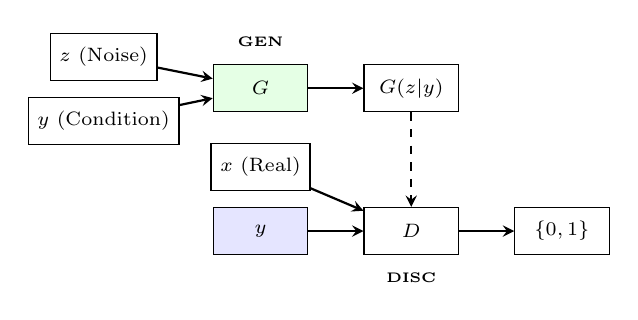
\begin{tikzpicture}[
        node distance=0.5cm,
        box/.style={draw, rectangle, minimum width=1.2cm, minimum height=0.6cm, font=\scriptsize},
        arrow/.style={->, >=stealth, thick}
    ]
    % Generator
    \node[box] (z) {$z$ (Noise)};
    \node[box, below=0.2cm of z] (y) {$y$ (Condition)};
    \node[box, right=0.7cm of z, yshift=-0.4cm, fill=green!10] (g) {$G$};
    \node[box, right=0.7cm of g] (gout) {$G(z|y)$};

    % Discriminator
    \node[box, below=1.2cm of gout] (d) {$D$};
    \node[box, left=0.7cm of d, fill=blue!10] (y2) {$y$};
    \node[box, above=0.2cm of y2] (x) {$x$ (Real)};
    \node[box, right=0.7cm of d] (dout) {$\{0, 1\}$};

    % Arrows
    \draw[arrow] (z) -- (g); \draw[arrow] (y) -- (g);
    \draw[arrow] (g) -- (gout);
    \draw[arrow] (x) -- (d); \draw[arrow] (y2) -- (d);
    \draw[arrow] (d) -- (dout);
    \draw[arrow, dashed] (gout) -- (d);

    \node[above=0.1cm of g, font=\tiny\bfseries] {GEN};
    \node[below=0.1cm of d, font=\tiny\bfseries] {DISC};
    \end{tikzpicture}
    }
    \end{column}
\end{columns}

\end{frame}

\begin{frame}{StyleGAN Series Evolution \cite{karras2019stylegan, karras2020stylegan2, karras2021stylegan3}}
\begin{columns}
\begin{column}{0.5\textwidth}
\begin{block}{StyleGAN (2019)}
\begin{itemize}
    \item Style-based generator
    \item AdaIN (Adaptive Instance Norm)
    \item Stochastic variation via noise
\end{itemize}
\end{block}

\begin{block}{StyleGAN2 (2020)}
\begin{itemize}
    \item Fixed artifacts (water droplets)
    \item Path length regularization
    \item No progressive growing
\end{itemize}
\end{block}
\end{column}

\begin{column}{0.5\textwidth}
\begin{block}{StyleGAN3 (2021)}
\begin{itemize}
    \item Aliasing-free architecture
    \item Equivariance to transformations
    \item Better interpolation
\end{itemize}
\end{block}

\begin{figure}
\centering
\includegraphics[width=0.8\textwidth]{images/stylegan_evolution.png}
\caption{Improvements across StyleGAN versions}
\end{figure}
\end{column}
\end{columns}
\end{frame}

\section{State-of-the-Art Applications}
\begin{frame}{Image Generation: BigGAN \cite{brock2018biggan}}
\begin{block}{Key Innovations}
\begin{itemize}
    \item \textbf{Scale}: Large batch sizes (2048) and models
    \item \textbf{Orthogonal Regularization}: Stabilize training
    \item \textbf{Truncation Trick}: Trade diversity for quality
\end{itemize}
\end{block}

\[
R_\beta(W) = \beta \|W^\top W - I\|_F^2
\]

\begin{figure}
\centering
\includegraphics[width=0.7\textwidth]{images/biggan_samples.png}
\caption{BigGAN samples at 512×512 resolution}
\end{figure}

\begin{alertblock}{Scaling Laws}
Performance $\propto$ (Model Size × Batch Size × Dataset Size)
\end{alertblock}
\end{frame}

%\begin{frame}{Text-to-Image Synthesis}
%\begin{columns}
%\begin{column}{0.5\textwidth}
%\begin{block}{DALL-E 2 \cite{ramesh2022hierarchical}}
%\begin{itemize}
%    \item Diffusion prior + decoder
%    \item CLIP embeddings
%    \item High semantic alignment
%\end{itemize}
%\end{block}
%
%\begin{block}{Stable Diffusion \cite{rombach2022high}}
%\begin{itemize}
%    \item Latent diffusion
%    \item Open source
%    \item Fine-grained control
%\end{itemize}
%\end{block}
%\end{column}
%
%\begin{column}{0.5\textwidth}
%\begin{figure}
%\centering
%\includegraphics[width=\textwidth]{images/text_to_image.png}
%\caption{"An astronaut riding a horse in photorealistic style"}
%\end{figure}
%
%\begin{block}{Imagen \cite{saharia2022imagen}}
%\begin{itemize}
%    \item T5-XXL text encoder
%    \item Cascade diffusion
%    \item State-of-the-art FID
%\end{itemize}
%\end{block}
%\end{column}
%\end{columns}
%\end{frame}

\begin{frame}{Text-to-Image Synthesis: Proprietary Models}
\begin{columns}[T]
    \begin{column}{0.5\textwidth}
    \begin{block}{DALL-E 2 \cite{ramesh2022hierarchical}}
    \begin{itemize}
        \item Diffusion prior + decoder
        \item CLIP embeddings
        \item High semantic alignment
    \end{itemize}
    \end{block}

    \begin{block}{Imagen \cite{saharia2022imagen}}
    \begin{itemize}
        \item T5-XXL text encoder
        \item Cascade diffusion
        \item State-of-the-art FID
    \end{itemize}
    \end{block}
    \end{column}

    \begin{column}{0.5\textwidth}
    \begin{figure}
    \centering
    % Scaling the image to ensure it fits the column height
    \includegraphics[width=0.9\textwidth, height=0.4\textheight, keepaspectratio]{images/text_to_image.png}
    \caption{"An astronaut riding a horse"}
    \end{figure}
    \end{column}
\end{columns}
\end{frame}


\begin{frame}{Text-to-Image Synthesis: Stable Diffusion}
\begin{block}{Stable Diffusion \cite{rombach2022high}}
\begin{itemize}
    \item \textbf{Latent Diffusion Model (LDM)}: Operates in a compressed $z$-space.
    \item \textbf{Efficiency}: Drastically reduces VRAM usage vs. pixel-space models.
    \item \textbf{Conditioning}: Flexible integration of text via Cross-Attention.
\end{itemize}
\end{block}

\begin{figure}
\centering
\resizebox{0.95\textwidth}{!}{
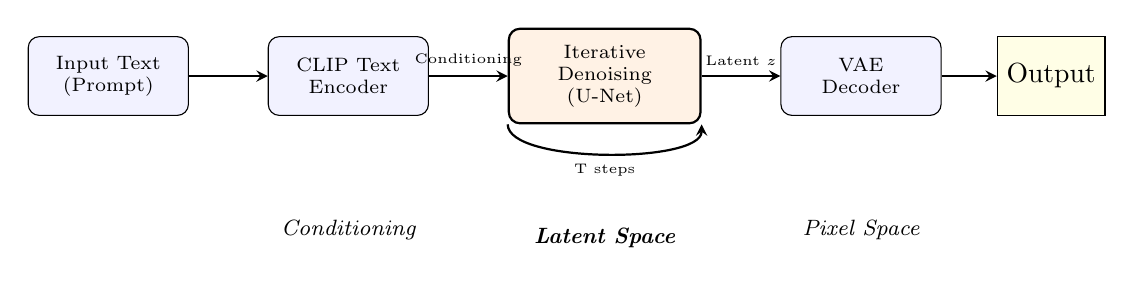
\begin{tikzpicture}[
    node distance=0.7cm and 1.0cm,
    block/.style={rectangle, draw, fill=blue!5, text width=1.8cm, align=center, rounded corners, minimum height=1cm, font=\scriptsize},
    latent/.style={rectangle, draw, fill=orange!10, text width=2.2cm, align=center, rounded corners, minimum height=1.2cm, font=\scriptsize, thick},
    arrow/.style={->, >=stealth, thick}
]

% Nodes
\node[block] (text) {Input Text\\(Prompt)};
\node[block, right=of text] (encoder) {CLIP Text\\Encoder};
\node[latent, right=of encoder] (unet) {Iterative\\Denoising\\(U-Net)};
\node[block, right=of unet] (vae) {VAE\\Decoder};
\node[draw, fill=yellow!10, minimum size=1cm, right=0.7cm of vae] (img) {Output};

% Connections
\draw[arrow] (text) -- (encoder);
\draw[arrow] (encoder) -- node[above, font=\tiny] {Conditioning} (unet);
\draw[arrow] (unet) -- node[above, font=\tiny] {Latent $z$} (vae);
\draw[arrow] (vae) -- (img);

% Corrected Loop arrow for denoising (Removed the 'midpoint' error)
\draw[arrow] (unet.south west) .. controls +(0,-0.5) and +(0,-0.5) .. (unet.south east) 
      node[below, pos=0.5, font=\tiny] {T steps};

% Labels for spaces
\node[below=1.2cm of encoder, font=\footnotesize\itshape] {Conditioning};
\node[below=1.2cm of unet, font=\footnotesize\itshape\bfseries] {Latent Space};
\node[below=1.2cm of vae, font=\footnotesize\itshape] {Pixel Space};

\end{tikzpicture}
}
\caption{The Stable Diffusion Pipeline: Conditioning $\to$ Latent Denoising $\to$ Reconstruction}
\end{figure}
\end{frame}


\begin{frame}{Medical Applications}
\begin{columns}
\begin{column}{0.5\textwidth}
\begin{block}{Data Augmentation}
\begin{itemize}
    \item Generate rare disease cases
    \item Balance imbalanced datasets
    \item Improve classifier robustness
\end{itemize}
\end{block}

\begin{block}{Anomaly Detection}
\begin{itemize}
    \item Learn normal distribution
    \item Flag deviations as anomalies
    \item Early disease detection
\end{itemize}
\end{block}
\end{column}

\begin{column}{0.5\textwidth}
\begin{figure}
\centering
\includegraphics[width=0.9\textwidth]{images/medical_gan.png}
\caption{Generated MRI scans for data augmentation}
\end{figure}

\begin{alertblock}{Ethical Considerations}
\begin{itemize}
    \item Patient privacy
    \item Validation requirements
    \item Clinical approval needed
\end{itemize}
\end{alertblock}
\end{column}
\end{columns}
\end{frame}

\section{Advanced Topics and Research Frontiers}
\begin{frame}{Diffusion Models vs GANs}
\begin{table}
\centering
\begin{tabular}{lcc}
\toprule
\textbf{Aspect} & \textbf{GANs} & \textbf{Diffusion Models} \\
\midrule
Training Stability & Low & High \\
Sample Quality & Excellent & Excellent \\
Sample Diversity & Good & Excellent \\
Training Speed & Fast & Slow \\
Sampling Speed & Fast & Slow \\
Mode Coverage & Partial & Full \\
Theoretical Understanding & Limited & Good \\
\bottomrule
\end{tabular}
\caption{Comparison of GANs and Diffusion Models (2023)}
\end{table}

\begin{block}{Hybrid Approaches}
\begin{itemize}
    \item GANs for fast sampling
    \item Diffusion for training stability
    \item Best of both worlds
\end{itemize}
\end{block}
\end{frame}

\begin{frame}{Ethical Considerations}
\begin{columns}
\begin{column}{0.5\textwidth}
\begin{alertblock}{Deepfakes}
\begin{itemize}
    \item Face swapping
    \item Voice cloning
    \item Misinformation risks
\end{itemize}
\end{alertblock}

\begin{alertblock}{Bias Amplification}
\begin{itemize}
    \item Dataset biases $\rightarrow$ model biases
    \item Underrepresentation issues
    \item Fairness concerns
\end{itemize}
\end{alertblock}
\end{column}

\begin{column}{0.5\textwidth}
\begin{block}{Mitigation Strategies}
\begin{itemize}
    \item \textbf{Watermarking}: Embed invisible markers
    \item \textbf{Detection}: Train classifiers to detect fakes
    \item \textbf{Attribution}: Track model origins
    \item \textbf{Regulation}: Legal frameworks
\end{itemize}
\end{block}

\begin{exampleblock}{Responsible AI Practices}
\begin{itemize}
    \item Transparency in generation
    \item Bias audits
    \item Ethical guidelines
\end{itemize}
\end{exampleblock}
\end{column}
\end{columns}
\end{frame}

\begin{frame}{Future Directions}
\begin{columns}
\begin{column}{0.5\textwidth}
\begin{block}{3D Generation}
\begin{itemize}
    \item Neural radiance fields (NeRF)
    \item 3D-aware GANs
    \item Multi-view consistency
\end{itemize}
\end{block}

\begin{block}{Video Synthesis}
\begin{itemize}
    \item Temporal consistency
    \item Long-term dependencies
    \item Story generation
\end{itemize}
\end{block}
\end{column}

\begin{column}{0.5\textwidth}
\begin{block}{Multimodal Generation}
\begin{itemize}
    \item Text + Image + Audio
    \item Cross-modal retrieval
    \item Unified representations
\end{itemize}
\end{block}

\begin{block}{Theoretical Advances}
\begin{itemize}
    \item Better convergence guarantees
    \item Optimal architectures
    \item Generalization bounds
\end{itemize}
\end{block}
\end{column}
\end{columns}

\begin{alertblock}{Grand Challenge}
\textbf{AGI-level creativity}: Systems that can generate truly novel, valuable content across domains.
\end{alertblock}
\end{frame}

\begin{frame}{Conclusion}
\begin{block}{Key Takeaways}
\begin{enumerate}
    \item GANs revolutionized generative modeling through adversarial training
    \item Theoretical foundation: Minimax game optimizing JS/Wasserstein distance
    \item Practical challenges: Instability, mode collapse → many solutions (WGAN, StyleGAN, etc.)
    \item State-of-the-art: Photorealistic image generation, many applications
    \item Active research: 3D/video generation, ethical considerations, hybrid models
\end{enumerate}
\end{block}

\begin{exampleblock}{Resources for Further Study}
\begin{itemize}
    \item \href{https://github.com/nashory/gans-awesome-applications}{Awesome GAN Applications}
    \item \href{https://arxiv.org/abs/1701.00160}{Original GAN paper}
    \item \href{https://www.deeplearning.ai}{DeepLearning.AI GAN Specialization}
\end{itemize}
\end{exampleblock}
\end{frame}

%\begin{frame}{References}
%\bibliographystyle{unsrt}
%\bibliography{gan_references}
%\end{frame}


% The [allowframebreaks] option will automatically create 
% "References I", "References II", etc.
\begin{frame}[allowframebreaks]{References}
    % Specify the style for numbered citations in order of appearance
    \bibliographystyle{unsrt}
    
    % Shrink text size to fit more references per page
    \footnotesize 
    
    % The bibliography command itself
    % This will only pull in items you have actually \cite{}'d
    \bibliography{gan_references}
\end{frame}

\end{document}